\documentclass[12pt]{article}

\usepackage{tikz}
\usepackage{amsmath,amsfonts,amssymb}
\usepackage{graphicx}
\usepackage{hyperref}
\usepackage{listings}
\usepackage{tikz}
\usepackage{ulem}
\usetikzlibrary{positioning,shapes,fit}
\usepackage{geometry}
\usepackage[justification=centering]{caption}
\usetikzlibrary{positioning,shapes}


\author{Aur\`ele Barri\`ere}
\title{LRC DM 1}
\date{February 3, 2017}

\def\exercise#1{\ \vspace{1cm}\\\Large\textbf{Exercise #1}\normalsize\\}
\def\question#1{\ \vspace{1cm}\\\textbf{Question #1:}\quad}

\def\tableau{
  \begin{figure}
    \centering
    \begin{tikzpicture}[%
        ->,
        shorten >=2pt,
        %>=stealth,
        node distance=0.8cm,
        noname/.style={%
          ellipse,
          minimum width=5em,
          minimum height=3em,
          draw
          ,thick,scale=0.4, every node/.style={transform shape}
        }
      ]
      \node[rectangle] (1) {$l\quad \neg((\Box p \wedge \Diamond q) \rightarrow \Diamond(p \wedge q))$};
      \node[rectangle] (2) [below=of 1] {\begin{tabular}{c}$l\quad \Box p\wedge\Diamond q$\\$l\quad\neg\Diamond(p\wedge q)$\end{tabular}};
      \node[rectangle] (3) [below=of 2] {$l\quad\Box(\neg p \vee \neg q)$};
      \node[rectangle] (4) [below=of 3] {\begin{tabular}{c}$l\quad\Box p$\\$l\quad\Diamond q$\end{tabular}};
      \node[rectangle] (5) [below=of 4] {\begin{tabular}{c}$R\ l\ l'$\\$l'\quad q$\end{tabular}};
      \node[rectangle] (6) [below=of 5] {$l'\quad p$};
      \node[rectangle] (7) [below=of 6] {$l'\quad \neg p \vee \neg q$};
      \node[rectangle] (8) [below left=of 7] {\begin{tabular}{c}$l'\quad\neg p$\\Contradictory\end{tabular}};
      \node[rectangle] (9) [below right=of 7] {\begin{tabular}{c}$l'\quad\neg q$\\Contradictory\end{tabular}};

      \path (1) edge [above] node {} (2)
      (2) edge [above] node {} (3)
      (3) edge [above] node {} (4)
      (4) edge [above] node {} (5)
      (5) edge [above] node {} (6)
      (6) edge [above] node {} (7)
      (7) edge [above] node {} (8)
      (7) edge [above] node {} (9);
      
  \end{tikzpicture}%
  \end{figure}
}



\def\tabdeux{
  \begin{figure}
    \centering
    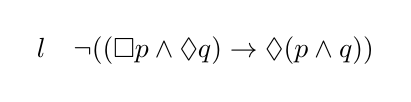
\begin{tikzpicture}[%
        ->,
        shorten >=2pt,
        %>=stealth,
        node distance=0.8cm,
        noname/.style={%
          ellipse,
          minimum width=5em,
          minimum height=3em,
          draw
          ,thick,scale=0.4, every node/.style={transform shape}
        }
      ]
      \node[rectangle] (1) {$l\quad \neg((\Box p \wedge \Diamond q) \rightarrow \Diamond(p \wedge q))$};
    \end{tikzpicture}
  \end{figure}
}

\begin{document}
\maketitle

\exercise{1}
\question{1} 
We show that the two Kripke models are bisimilar by giving a bisimulation relation between the two.
Let $R_{a1}, R_{b1}$ be the accessibility relations of the first Kripke model, and $R_{a2}, R_{b2}$ the accessibility relations of the second one.

Consider $Z$ the following binary relation :
$$\left\{
\begin{array}{l}
\forall n\in\mathbb{N},\quad w\ Z\ w^n \\
\forall n\in\mathbb{N},\quad v\ Z\ v^n
\end{array} 
\right.$$

Let's show that the relation $Z$ is a bisimulation.
\paragraph{Atom} Every world in each Kripke model make true the same propositional letter  : $p$, and only this one. 

\paragraph{Forth} Let $n\in\mathbb{N}$. We have $w\ Z\ w^n$. The only successor of $w$ in the first Kripke model is $v$ : $w\ R_{a1}\ v$. We also have $w^n\ R_{a2}\ v^n$. And by definition of $Z$, $v\ Z\ v^n$.

Let $n\in\mathbb{N}$. We have $v\ Z\ v^n$. The only successor of $v$ in the first Kripke model is $w$ : $v\ R_{b1}\ w$. We also have $v^n\ R_{b2}\ w^{n+1}$. And by definition of $Z$, $w\ Z\ v^{n+1}$.

Thus, the \textit{Forth} rule is true for $Z$, as every pair in relation with $Z$ is either $w\ Z\ w^n$ or $v\ Z\ v^n$ by definition.

\paragraph{Back} Let $n\in\mathbb{N}$. We have $w\ Z\ w^n$. The only successor of $w^n$ in the first Kripke model is $v^n$. We also have $w\ R_{a1}\ v$ and $v\ Z\ v^n$. 

 Let $n\in\mathbb{N}$. We have $v\ Z\ v^n$. The only successor of $v^n$ in the first Kripke model is $w^{n+1}$. We also have $v\ R_{b1}\ w$ and $w\ Z\ w^{n+1}$. 

\paragraph{Conclusion} $Z$ is a non-empty bisimulation between the two Kripke models. The two Kripke models are thus bisimilar.


\question{2} The smallest Kripke model bisimilar to $\mathcal{M}$ must have at least one world, for the bisimulation to be non-empty.

The Kripke model with only one world in which the propositional letter $t$ is true is bisimilar to $\mathcal{M}$. Let $w$ be this world.

We then define $Z$ the bisimulation such that $9\ Z\ w$. $Z$ is a bisimulation : in both $9$ and $w$, only $t$ is true, and both $9$ and $w$ have no successors. And this Kripke model is the smallest possible as it only has one world.

The Kripke contraction is thus $(\{w\},\emptyset,V)$ such that $V(w,t)=\mathit{true}$.


\question{3}

\paragraph{Union of two bisimulations} We will first prove that the union of two bisimulations is a bisimulation.
Let $Z_1$ and $Z_2$ be two bisimulations between $\mathcal{M}$ and $\mathcal{M}'$. Let $Z=Z_1\cup Z_2$.

\textit{Atom} is true for $Z$. Indeed, whenever $w\ Z\ v$, either $w\ Z_1\ v$ or $w\ Z_2\ v$. In each case, we have that $w$ and $v$ make true the same propositional letters because $Z_1$ and $Z_2$ are bisimulations.

\textit{Forth} is true for $Z$. Consider the case where $w\ Z_1\ v$ (the case with $Z_2$ is the same). In that case, forall $w'$ such that $w\ R\ w'$, there exists some $v'$ such that $v\ R\ v'$ and $w'\ Z_1\ v'$. Then by definition of $Z$, we also have $w'\ Z\ v'$.
\textit{Back} is also true for $Z$ : the proof is symmetrical.

Thus, $Z$ is a bisimulation between $\mathcal{M}$ and $\mathcal{M}'$.

\paragraph{Finite number of bisimulations} Then, we show that between two finite Kripke frames, there exists only a finite number of bisimulation. Indeed, a bisimulation is included in the set $\mathcal{W}^\mathcal{M}\times\mathcal{W}^\mathcal{M'}$, which is finite.

\paragraph{Union of bisimulations} We can now deduce that any non-empty union of bisimulations is a bissimulation recursively on the number of bisimulations in the collection. Since this number is finite, and because the union of two bisimulations is one too, then we have that the union of the whole collection is a bisimulation as well.

\paragraph{Maximal bisimulation} Let $Z_m = \underset{X \mathit{bisimulation}}{\bigcup} X$. The union is finite because there only is a finite number of bisimulation. There is always at least one bisimulation between two Kripke models : $\emptyset$. We can thus apply the previous result and deduce that $Z_m$ is a bisimulation. Moreover, for each bisimulation $X$, by definition of $Z_m$, we have $X\subseteq Z_m$. Thus, $Z_m$ is a maximal bisimulation.



\exercise{2}
\question{1}
\paragraph{Tableau method}

\tableau
\tabdeux
\end{document}
